\documentclass[11pt]{article}
\usepackage[english]{babel}
\linespread{1.0}
\usepackage{slantsc}
\usepackage[hmargin=1in,vmargin=3cm]{geometry}
%\input{./bild_mk2.sty}
\ProvidesPackage{default}
% common packages etc for stuff
\usepackage{extract}
\usepackage{fancyhdr}
\usepackage[utf8x]{inputenc}
\usepackage[LGR,T1,OT1]{fontenc}
\usepackage[svgnames,x11names]{xcolor} 
\usepackage{amsfonts}
\usepackage{amssymb}
\usepackage{mathtools}
\usepackage{graphicx}
\usepackage{setspace}
\usepackage{tabularx}
\usepackage{fancybox}
\usepackage{array}
\usepackage{multirow}
\usepackage{framed}
\usepackage{float}
\usepackage{color}
\usepackage{booktabs}
\usepackage[version=4,arrows=pgf]{mhchem}
\usepackage{microtype}
\usepackage{cancel}
\usepackage{marvosym}
\usepackage{fontawesome}
\usepackage{lettrine} 
\usepackage{tikz}
\usepackage{ctable}
\usepackage{simplewick}
\usepackage[full]{textcomp} 
\usepackage{tabulary}
\usepackage{enumitem}
\usepackage{easylist}
\usepackage[italicdiff]{physics}
\usepackage{xparse}
\usepackage[normalem]{ulem}
\usepackage[labelfont=bf,sf,textfont=up,labelsep=period]{caption} 
\usepackage{pgfplots}
%\usepackage{tocstyle}
\setlist{noitemsep}
\setlist[itemize,2]{label=$\triangleright$}
\setlist[itemize,3]{label=\textopenbullet}
\setlist[enumerate,1]{label=\arabic*., ref=\arabic*}
\setlist[enumerate,2]{label=(\alph*), ref=\theenumi.\alph*}
\setlist[enumerate,3]{label=(\roman*), ref=\theenumii.\roman*}
\setlist[description]{font=\sffamily\bfseries,style=nextline}
\newlist{romanenum}{enumerate}{3}
\setlist[romanenum, 1]{labelindent=\parindent,leftmargin=*,label=\Roman*.,align=left}
\setlist[romanenum, 2]{label=\roman*.}
\setlist[romanenum, 3]{label=\alph*)}
\newlist{boxenum}{enumerate}{1}
\setlist[boxenum]{label=\fbox{\arabic*}}


\definecolor{EmphGreen}{HTML}{007d5e}
\definecolor{InorganicGreen}{HTML}{007d5e}
\definecolor{InorganicBlue}{HTML}{37698a}
\definecolor{InorganicOrange}{HTML}{a15230}
\definecolor{NeptuneBlue}{HTML}{16709d}
\definecolor{darkblue}{RGB}{47,68,117}
\definecolor{AlmostBlack}{RGB}{38,38,38}
\definecolor{NearBlack}{RGB}{26,26,26}
\definecolor{lightgray}{gray}{0.95}

\definecolor{MplBlue}{HTML}{1f77b4}
\definecolor{MplOrange}{HTML}{ff7f0e}
\definecolor{MplGreen}{HTML}{2ca02c}
\definecolor{MplRed}{HTML}{d62728}
\definecolor{MplPurple}{HTML}{9467bd}
\definecolor{MplGrey}{HTML}{7f7f7f}
\definecolor{MplYellow}{HTML}{bcbd22}
\definecolor{MplCyan}{HTML}{17becf}


\usepackage{titlecaps}
\usepackage[explicit]{titlesec}
\usepackage{titletoc}
\titleformat{\section}{\Large\sffamily\bfseries}{\thesection. }{1.5ex}{#1}
\titleformat{\subsection}{\large\sffamily\bfseries}{\thesubsection. }{1.0ex}{#1}
\titleformat{\subsubsection}{\sffamily\bfseries}{\thesubsubsection\ }{0.5ex}{#1}
\titlespacing*{\section}{0em}{1.0em}{0.5em}
\titlespacing*{\subsection}{0em}{1.0em}{0.5em}
\titlespacing*{\subsubsection}{0pt}{0.5em}{0.5em}

\pagestyle{fancyplain}
\renewcommand{\headrulewidth}{0pt}
\fancyhf{}
\fancyfoot[R]{\thepage} 
\renewcommand{\title}[3]{\begin{flushleft}\LARGE\sffamily\bfseries{#1}\\[1ex] 
    \normalfont\sffamily \large #2 \hfill \normalsize #3 \end{flushleft}}

\usepackage{hyperref}
\hypersetup{colorlinks=true,linkcolor=Black,citecolor=Black,urlcolor=MplBlue}
\newcommand{\ds}{\displaystyle}
\renewcommand{\vec}[1]{\harpoonacc{#1}}
\renewcommand{\t}{\dagger}
\newcommand{\cip}[2]{\left(#1\middle|#2\right)\:}
\newcommand{\cmel}[3]{\left(#1 \middle| #2 \middle| #3 \right)\:}
\newcommand{\Coul}{\mathcal{J}}
\newcommand{\Exch}{\mathcal{K}}
\newcommand{\coverb}[2]{\overbrace{#1}^{\mathclap{#2}}}
\newcommand{\cunderb}[2]{\underbrace{#1}_{\mathclap{#2}}}


\numberwithin{equation}{section}

\usetikzlibrary{matrix,arrows,arrows.meta,positioning,decorations.pathmorphing,
decorations.pathreplacing,decorations.markings,shapes,calc,through,intersections,
backgrounds,patterns,shadings,bending,fit,petri,fadings}

\tikzset{
%        with arrow/.style={
%                decoration={
%                        markings,
%                        mark=at position #1 with {
%                                \node[
%                                transform shape,
%                                xshift=-0.5mm,
%                                fill,
%                                inner sep=1pt,
%                                draw=none,
%                                dart
%                                ] { };
%                                },
%                },
%                postaction={
%                        decorate=true,
%                        },
%        },
%        with reversed arrow/.style={
%                decoration={
%                        markings,
%                        mark=at position #1 with {
%                                \node[
%                                transform shape,
%                                xshift=-0.5mm,
%                                rotate=180,
%                                fill,
%                                inner sep=1pt,
%                                draw=none,
%                                dart
%                                ] {};
%                                        },
%                                },
%                postaction={
%                        decorate=true,
%                        },
%        },
%        internal line/.style={
%                draw=none,
%                decoration={name=none},
%                postaction={
%                        draw,
%                        with arrow=0.5,
%                },
%                thick,
%        },
%        external line/.style={
%                draw=none,
%                decoration={name=none},
%                postaction={
%                        draw,
%                        with reversed arrow=0.5,
%                },
%                thick,
%        },
%        internal loop/.style={
%                draw=none,
%                decoration={name=none},
%                postaction={
%                        draw,
%                        with arrow=0.75,
%                },
%                thick,
%        },
%        top loop/.style={
%                draw=none,
%                decoration={name=none},
%                postaction={
%                        draw,
%                        with arrow=0.25,
%                },
%                thick,
%        },
%        fermion/.style={
%                draw=none,
%                decoration={name=none},
%                postaction={
%                        draw,
%                        with arrow=0.5,
%                },
%                thick,
%        },
%        anti fermion/.style={
%                draw=none,
%                decoration={name=none},
%                postaction={
%                        draw,
%                        with reversed arrow=0.5,
%                },
%                thick,
%        },
%        shift fermion/.style={
%                draw=none,
%                decoration={name=none},
%                postaction={
%                        draw,
%                        with arrow=0.25,
%                },
%                thick,
%        },
%        shift antifermion/.style={
%                draw=none,
%                decoration={name=none},
%                postaction={
%                        draw,
%                        with reversed arrow=0.25,
%                },
%                thick,
%        },
%        exchange/.style={
%                draw=none,
%                decoration={name=none},
%                postaction={
%                        draw,
%                        with arrow=0.0,
%                },
%                thick,
%        },
%        loopfermion/.style={
%                draw=none,
%                decoration={name=none},
%                postaction={
%                        draw,
%                        with arrow=0.75,
%                },
%                thick,
%        },
%        loopantifermion/.style={
%                draw=none,
%                decoration={name=none},
%                postaction={
%                        draw,
%                        with reversed arrow=0.75,
%                },
%                thick,
%        },
%        resolvant/.style={
%                draw,
%                circle,
%                minimum width=3mm,
%                inner sep=0pt,
%                label={[font=\tiny]center:$ 1 $}
%        },
%        ZN operator/.style={
%                -{Rays[length=8pt,width=8pt]},
%                dashed,
%                semithick
%        },
%        QN operator/.style={
%                isosceles triangle,draw,thick,rotate=90,anchor=apex,minimum height=2.5mm, minimum width=3.5mm,inner sep=0pt,isosceles triangle stretches,fill=white
%        },
%        hole/.style={
%                circle,
%                fill=Black,
%                inner sep=0pt,
%                minimum width=1.2mm
%        },
%        block/.style={
%                draw,
%                thick,
%                pattern=north east lines,
%                pattern color=Black,
%                rectangle,
%                rounded corners,
%                minimum height = 1.3em,
%                minimum width = 1.3em
%        },
%        open/.style={
%                draw,
%                thick,
%                pattern=north east lines,
%                pattern color=Black, circle,
%                minimum height = 1.1em,
%                minimum width = 1.1em
%        },
	every line/.style={
		rounded corners,
		thick},
%        C2 operator/.style={
%                draw,
%                thick,
%                pattern=north east lines,
%                pattern color=Black,
%                rectangle,
%                minimum height = 1.9cm,
%                minimum width = 0.27cm,
%                rounded corners
%        },
%        Z operator/.style={
%                -{Rays[
%                        length=8pt,
%                        width=8pt
%                        ]
%                },
%                semithick,
%                decorate,
%                decoration={
%                        snake,
%                        amplitude=.4mm,
%                        segment length=3mm,
%                        post length=0.18mm
%                }
%        },
        >={
                Stealth[]
        },
%        particle/.style={
%                shade,
%                inner sep=0pt,
%                circle,
%                ball color=MplGreen!80,
%                minimum width=4mm,
%                },
%        electron/.style={
%                shade,
%                inner sep=0pt,
%                circle,
%                ball color=MplBlue!80,
%                minimum width=3mm,
%                },
%        level/.style={
%                fill=black,
%                inner sep=0pt,
%                minimum width=0.8cm,
%                minimum height=0.4mm,
%        },
%        carbon/.style={
%                shade,
%                inner sep=0.8pt,
%                outer sep=0.5pt,
%                circle,
%                ball color=ModernGrey!80,
%                minimum width=3.25mm,
%                },
%        hydrogen/.style={
%                shade,
%                inner sep=0.3pt,
%                outer sep=0.5pt,
%                circle,
%                ball color=ModernGrey!20,
%                minimum width=2mm,
%                },
%        nitrogen/.style={
%                shade,
%                inner sep=0.8pt,
%                outer sep=0.5pt,
%                circle,
%                ball color=MplBlue!80,
%                minimum width=3mm,
%                },
%        ghost area/.style={
%                fill=white,
%                inner sep=0.5pt,
%                outer sep=0.5pt,
%                minimum width=3.25mm,
%                minimum height=3.25mm,
%                },
%        level2/.style={
%                fill=black,
%                inner sep=0pt,
%                minimum width=0.8cm,
%                minimum height=0.4mm,
%                },
}

\newcommand{\meanface}{
\begin{tikzpicture}
    \begin{scope}[scale=0.5]
     \node[shape=circle,minimum size=4ex,outer sep=0pt,draw,semithick,scale=0.5,inner sep=0pt] (err) {};
      \fill[shift={( 0.6ex,0.3ex)},rotate=90] (0,0) ellipse (0.30ex and 0.25ex);
      \fill[shift={(-0.6ex,0.3ex)},rotate=90] (0,0) ellipse (0.30ex and 0.25ex);
      \draw[semithick] (-0.9ex,-1.0ex)..controls
          (-0.5ex,-0.5ex)and(0.5ex,-0.5ex)..(0.9ex,-1.0ex);
      \draw[semithick] ( 0.2ex,0.85ex) to ++(30:0.85ex);
      \draw[semithick] (-0.2ex,0.85ex) to ++(150:0.85ex);
   \end{scope}
\end{tikzpicture}
}     
%%%%%%%%%%% MATHEMATICS %%%%%%%%%%%%%%%
%\DeclareMathSymbol{\umu}{\mathalpha}{operators}{0}
%\DeclareMathOperator{\sumint}{\sumint}

\newcommand*{\plogo}{\fbox{${\mathscr{L}}_\text{\Sun}^{\mathscr{A}}$}} 
\newcommand{\del}{\nabla}
\newcommand{\tphi}{\ensuremath{\widetilde{\Phi}}}
\newcommand{\dye}{\partial}
\newcommand{\vf}{\varphi}
\newcommand{\ve}{\varepsilon}
\newcommand{\vrho}{\varrho}
\newcommand{\vk}{\varkappa}
\newcommand{\vth}{\vartheta}
%\newcommand{\k}{\kappa}

\newcommand{\Hm}{\mathscr{H}}
\newcommand{\SE}{Schr\"{o}dinger equation}
\newcommand{\qsum}[2]{\sum_{#1}^{#2}}
\newcommand{\dir}[2]{\left\langle #1\middle| #2 \right\rangle}
\newcommand{\qavg}[3]{\left\langle #1 \middle| #2\middle| #3 \right\rangle}
\newcommand{\ipm}[2]{\big\langle #1\big| #2 \big\rangle}
\newcommand{\melm}[3]{\big\langle #1 \big| #2 \big| #3 \big\rangle}
\newcommand{\Rd}{\ensuremath{\mathscr{R}_{\varkappa}^{}}}
\newcommand{\ketm}[1]{\big| #1 \big\rangle}
\newcommand{\bram}[1]{\big\langle #1 \big|  }
\newcommand{\evm}[1]{\big\langle #1 \big\rangle}
\newcommand{\cbk}[1]{{\color{Crimson}\bm{\langle} {\color{Black}#1} \bm{\rangle} }}
\newcommand{\Bcbk}[1]{{\color{Crimson}\bm{\big\langle} {\color{Black}#1} \bm{\big\rangle}}}
\newcommand{\ncon}[1]{N\bigl[ #1 \bigr]}
\newcommand{\RWb}[1]{\big\{(R^{(0)}W)^{#1}\big\}}
\newcommand{\s}{^{}_}
\newcommand{\f}[2]{_{#1}^{#2}}
\newcommand{\ao}[1]{a_{#1}^{}}
\newcommand{\co}[1]{a_{#1}^{\dagger}}

\renewcommand{\t}{\dagger}
\newcommand{\HF}{Hartree-Fock}
\newcommand{\Ham}{Hamiltonian}
\newcommand{\KS}{Kohn-Sham}
\newcommand{\ort}{orthonormal}
\newcommand{\stp}{\cancel{p}}
\newcommand{\stq}{\cancel{q}}
\newcommand{\nmo}{N_{p}^{}}
\newcommand{\nmod}{N_{p}^{\dagger}}
\newcommand{\tsum}[2]{\sum_{\mathclap{\substack{#1}}}^{#2}}

\newcommand{\dpq}{\delta_{pq}^{}}
\newcommand{\dps}{\delta_{ps}^{}}
\newcommand{\oop}{\hat{o}}
\newcommand{\Oop}{\hat{O}}
\newcommand{\zo}{\hat{z}}
\newcommand{\z}{\hat{z}}
\renewcommand{\v}{\hat{v}}
\renewcommand{\H}{\hat{H}}
\renewcommand{\t}{\dagger}
\newcommand{\pkv}[1]{p_{k_{#1}^{}}^{}}
\newcommand{\pohq}{\langle p | \hat{\mathrm{o}}_1^{}|q \rangle}
\newcommand{\prov}{\Pi^{p_i^{}}X^{\dagger}|0\rangle}
\newcommand{\cb}[1]{\{ #1 \}}
\newcommand{\lrcb}[1]{\left\{ #1 \right\}}
\newcommand{\sld}[1]{\left|\left\{ #1 \right\} \right \rangle}
\newcommand{\ocp}[1]{\mathcal{#1}}
\newcommand{\seF}{\mathscr{F}_{s}^{}}
\newcommand{\heF}{\mathscr{H}_{s}^{}}

\newcommand{\rw}{\ensuremath{\rightarrow}}
\newcommand{\Rw}{\ensuremath{\Rightarrow}}
\newcommand{\lrw}{\ensuremath{\longrightarrow}}
\newcommand{\lw}{\ensuremath{\leftarrow}}
\newcommand{\Lw}{\ensuremath{\Leftarrow}}
\newcommand{\llw}{\ensuremath{\longleftarrow}}
\newtheorem{lemma}{Lemma}
\newcommand{\bx}{\ensuremath{\mathbf{x}}}
\newcommand{\fop}[1]{\mathscr{#1}}
\newcommand{\mb}[1]{\mathbf{#1}}
\newcommand{\lrp}[1]{\left( #1 \right)} 
\newcommand{\lrb}[1]{\left[ #1 \right]}
\newcommand{\tte}[1]{\text{#1}}
\newcommand{\bb}[1]{\textbf{#1}}

%%%%%%%%% Old commands for capability. Do not use. %%%%%%%%%%%%
\newcommand{\smls}[2]{{#1}_{#2}^{}}
\newcommand{\smlx}[2]{{{#1}_{ #2}^{}}}
\newcommand{\sls}[2]{{#1}_{#2}^{}}
\newcommand{\slx}[2]{{{#1}_{\! #2}^{}}}
\newcommand{\lrnp}[1]{\left( #1 \right)} 
\newcommand{\lrsb}[1]{\left[ #1 \right]}                  
%%%%%%%%%%%%%%%%%%%%%%%%%%%%%%%%%%%%%%%

\usepackage[largesc]{newtxtext}
\usepackage[scaled=0.85]{DejaVuSansMono}
\usepackage[vvarbb, nosymbolsc]{newtxmath}
\usepackage{multicol}
\usepackage[cal=esstix, scr=rsfso]{mathalfa}
\usepackage{bm}
\usepackage{verbatim}
%\numberwithin{equation}{section}
\renewcommand{\arraystretch}{1.0}
%\usepackage{titlecaps}
%\usepackage[explicit]{titlesec}
%\usepackage{titletoc}
%\titleformat{\section}{\Large\sffamily\bfseries}{\thesection. }{1.5ex}{#1}
%\titleformat{\subsection}{\large\sffamily\bfseries}{\thesubsection. }{1.0ex}{#1}
%\titleformat{\subsubsection}{\sffamily\bfseries}{\thesubsubsection\ }{0.5ex}{#1}
%\titlespacing*{\section}{0em}{1.0em}{0.5em}
%\titlespacing*{\subsection}{0em}{1.0em}{0.5em}
%\titlespacing*{\subsubsection}{0pt}{0.5em}{0.5em}
%
%\pagestyle{fancyplain}
%\renewcommand{\headrulewidth}{0pt}
%\fancyhf{} \fancyfoot[R]{\thepage}
%\renewcommand{\title}[3]{\begin{flushleft}\LARGE\sffamily\bfseries{#1}\\[1ex]
%    \normalfont\sffamily \large #2 \hfill \normalsize #3 \end{flushleft}}
%
%\usepackage{hyperref}
%\hypersetup{colorlinks=true,linkcolor=Black,citecolor=Black,urlcolor=MplBlue}
%\newcommand{\ds}{\displaystyle}
%\renewcommand{\vec}[1]{\harpoonacc{#1}}
%\renewcommand{\t}{\dagger}
%\newcommand{\cip}[2]{\left(#1\middle|#2\right)\:}
%\newcommand{\cmel}[3]{\left(#1 \middle| #2 \middle| #3 \right)\:}
%\newcommand{\Coul}{\mathcal{J}}
%\newcommand{\Exch}{\mathcal{K}}
%\newcommand{\coverb}[2]{\overbrace{#1}^{\mathclap{#2}}}
%\newcommand{\cunderb}[2]{\underbrace{#1}_{\mathclap{#2}}}
\begin{document}
\title{The SCF Workshop Notes 1}{Lucas Aebersold}{\today}
\setcounter{section}{2}
\subsection{How to Gaussian Integrate}
%pg 153 -> gbasis 
Let's take a quick step back and ask the very same question that dawned on me when learning about this stuff ``What is the actual mathematical form of the thing we're solving? I mean TF do I actually put into a code to compute this stuff''. Let's first refamiliarize ourselves with Gaussian basis sets, and then derive our expressions using Gaussian orbitals. 

In molecular calculations, you generally use a fixed molecular coordinate system, so that the basis functions are centered at position vectors $\bb{R}_A$. The value at a position vector $\bb{r}$, of a function centered at $\bb{R}_A$ will depend on $\bb{r} - \bb{R}_A$, thus we write a general basis function as $\phi_\mu (\bb{r} - \bb{R}_A)$ to denote that it is centered at $\bb{R}_A$
\begin{figure}[H]
	\centering
\begin{tikzpicture}[
hole/.style={
	circle,
	fill=Black,
	inner sep=0pt,
	minimum width=1.2mm
},
	empty/.style={
	inner sep=0pt,
	outer sep=0pt,
},
]

\draw[semithick] (0,0,0) to (0, 0, 3); 
\draw[semithick] (0,0,0) to (0, 3, 0); 
\draw[semithick] (0,0,0) to (3, 0, 0); 

\node[empty] (O) {}; 
\node[hole] (rRA) at ++(60:4cm) {};
\coordinate (Ac) at ++(30:3.0cm); 
\node[circle, ball color=MplBlue, opacity=0.3, minimum size=1.52cm] (E) at (Ac) {}; 

\node[hole,label=-30:$A$] (A) at ++(30:3.0cm) {};

%\draw[name path=AB] (A) to node[near end, hole, label=180:$P$] (P) {} (B); 
%\draw[name path=CD] (C) to node[near start, hole, label=0:$Q$] (Q) {} (D); 

\draw[->] (O) to node[auto, swap] {$\mathbf{R}_A$} (A);
\draw[->] (O) to node[auto] {$\mathbf{r}$} (rRA);
\draw[->] (A) to node[auto, swap] {$\mathbf{r} - \mathbf{R}_A$} (rRA);

\end{tikzpicture}
\caption{Coordinate system representation for the atom centered Gaussian}
\end{figure}
Our typical unnormalized Gaussian friend looks like
\begin{equation}\label{key}
\tilde{g}_{1s} (\bb{r} - \bb{R}_A) = e^{-\alpha | \bb{r} - \bb{R}_A|^2} 
\end{equation}
The normalized 1$s$ \textit{Gaussian-type function}, centered at $\bb{R}_A$, can be written as 
\begin{equation}\label{key}
\phi_{1s}^{\mathrm{GF}} (\alpha, \bb{r} - \bb{R}_A) = \qty(\frac{2\alpha}{\pi})^{3/4}e^{-\alpha|\bb{r} - \bb{R}_A|^2} 
\end{equation}
The integrals take the generic form 
\begin{equation}\label{}
\cip{\mu_A \nu_B}{\lambda_C \sigma_D}= \int \phi_\mu^{A*}(\bb{r}_1) \phi_\nu^{B}(\bb{r}_1) r_{12}^{-1} \phi_\lambda^{C*} (\bb{r}_2) \phi_\sigma^D (\bb{r}_2) \dd{\bb{r}_1 d\bb{r}_2} 
\end{equation}
which will involve taking the product of Gaussian functions, fortunately this product is just another Gaussian centered at the midpoint between the two other centers
\begin{equation}
\phi_{1s}^{\mathrm{GS}}(\alpha, \mathbf{r} - \mathbf{R}_A) \phi_{1s}^{\mathrm{GS}}(\beta, \mathbf{r} - \mathbf{R_B}) = K_{AB} \phi_{1s}^{\mathrm{GS}}(p, \mathbf{r}- \mathbf{R}_p)
\end{equation}
where this constant $K_{AB}$ is 
\begin{equation}\label{}
K_{AB} = \qty(\frac{2\alpha\beta}{(\alpha + \beta) \pi})^{3/4} \exp(-\frac{\alpha\beta}{\alpha + \beta}) \exp(|\mathbf{R}_A - \mathbf{R}_B|^2)
\end{equation}
The new exponent of the Gaussian centered at $\mathbf{R}_P$ is 
\begin{equation}\label{}
p = \alpha + \beta 
\end{equation}
and the third center $P$ is on a line joining the centers $A$ and $B$
\begin{equation}\label{key}
\mathbf{R}_P = (\alpha \mathbf{R}_A + \beta \mathbf{R}_B)/(\alpha + \beta) 
\end{equation}
\begin{figure}[H]
	\centering
	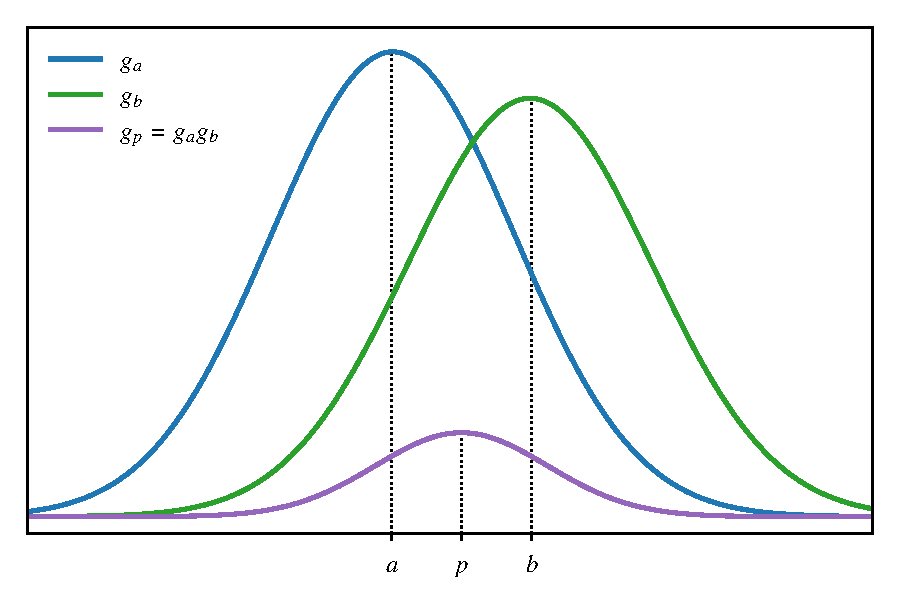
\includegraphics[width=0.5\textwidth]{gauss_overlaps}
	\caption{Product of two Gaussian} 
\end{figure}
\begin{equation}\label{}
\cip{\mu_A \nu_B}{\lambda_C \sigma_D}= K_{AB} K_{CD} \int \phi_{1s}^{\mathrm{GS}}(p, \mathbf{r}_1 - \bb{R}_p)r_{12}^{-1} \phi_{1s}^{\mathrm{GS}}(q, \bb{r}_2 - \bb{R}_Q) \dd{\bb{r}_1 d\bb{r}_2} 
\end{equation}
The formula for a series of Gaussian, known as contracted GFs is
\begin{equation}\label{key}
\phi_\mu^{\mathrm{CGF}}(\bb{r} - \bb{R}_A) = \sum_{p = 1}^L d_{p\mu} \phi_p^{\mathrm{GF}}(\alpha_{p\mu}, \bb{r} - \bb{R}_A) 
\end{equation}
where $d_{p\mu}$ are the contraction coefficients
\subsubsection{Integral Forms of 1s Gaussians}
The $\bb{S}$ overlap matrix has the basic form that when integrated gives us the following equation
\begin{align*}
S = \cip{A}{B} &= \int \tilde{g}_{1s}(\bb{r}_1 - \bb{R}_A)\tilde{g}_{1s}(\bb{r}_1 - \bb{R}_B) \dd{\bb{r}_1} \\
&= \qty(\frac{\pi}{(\alpha + \beta)})^{3/2} \exp(-\frac{\alpha\beta}{(\alpha + \beta)}|\bb{R}_A - \bb{R}_B|^2)
\end{align*}
Kinetic energy integral will give us this expression 
\begin{align*}
\cmel{A}{-\frac{1}{2}\laplacian }{B} &=\int \tilde{g}_{1s}(\bb{r}_1 - \bb{R}_A) (-\frac{1}{2}\laplacian) \tilde{g}_{1s}(\bb{r}_1 - \bb{R}_B) \dd{\bb{r}_1} \\
&= \frac{\alpha\beta}{(\alpha + \beta)} \left[ 3 - \frac{2\alpha\beta}{(\alpha + \beta)} | \bb{R}_A - \bb{R}_B|^2 \right]\left[\frac{\pi}{(\alpha + \beta)}\right]^{3/2} \exp(-\frac{\alpha\beta}{(\alpha + \beta)} |\bb{R}_A - \bb{R}_B|^2)
\end{align*}
For the nuclear attraction integral, I'm going to have to pull a Cukier and refer you to pg. 412--414 of S\&O for the exact derivation. 

During the derivation (which involves Fourier transforms!---you'll never escape them, submit to their study or perish), we end up needing to introduce the $F_0$ function, defined as
\begin{equation}\label{key}
F_0 (t) = t^{-1/2} \int_0^{t^{1/2}} e^{-y^2}\dd{y} 
\end{equation}
It is related to the error function by 
\begin{equation}\label{key}
F_0 (t) = \frac{1}{2} (\pi/t)^{1/2} \erf(t^{1/2}) 
\end{equation}
which itself is related to the Gamma function and so on, anyway, our nuclear attraction integral then becomes
\begin{equation}\label{key}
\cmel{A}{-\frac{Z_C}{r_{1C}^{
}}}{B} = -\frac{2\pi}{(\alpha + \beta)} Z_C \exp(-\frac{\alpha \beta}{(\alpha + \beta)}|\bb{R}_A - \bb{R}_B|^2) F_0\qty((\alpha + \beta)|\bb{R}_P - \bb{R}_C|^2)
\end{equation}
Now consider the horrid two-electron repulsion integral 
\begin{align*}
\cip{AB}{CD} &= \exp(-\frac{\alpha\beta}{(\alpha + \beta)} |\bb{R}_A - \bb{R}_B|^2 - \frac{\gamma \delta}{(\gamma + \delta)} |\bb{R}_C - \bb{R}_D|^2 ) \\
&\qquad \times \int \exp(-p|\bb{r}_1 - \bb{R}_P|^2) r_{12}^{-1} \exp(-q |\bb{r}_2 - \bb{R}_Q|^2) \dd{\bb{r}_1 d\bb{r}_2} \\
 &= \frac{2\pi^{5/2}}{(\alpha + \beta)(\gamma + \delta)(\alpha + \beta + \gamma + \delta)^{1/2}}\\
 &\qquad \times \exp(-\frac{\alpha\beta}{(\alpha + \beta)} |\bb{R}_A - \bb{R}_B|^2 - \frac{\gamma \delta}{(\gamma + \delta)} |\bb{R}_C - \bb{R}_D|^2) F_0 \qty(\frac{(\alpha + \beta)(\gamma + \delta)}{(\alpha + \beta + \gamma + \delta)} |\bb{R}_P - \bb{R}_Q|^2)
\end{align*}

\begin{figure}[H]
	\centering
	\begin{tikzpicture}[
	hole/.style={
		circle,
		fill=Black,
		inner sep=0pt,
		minimum width=1.2mm
	},
	]
	\node[hole,label=-60:$B$] (B) {}; 
	\node[hole,label=30:$A$] (A) at ++(80:3cm) {};
	
	\node[hole,label=0:$D$] (D) at ($(B) + (-10:4cm)$) {}; 
	\node[hole,label=30:$C$] (C) at ($(D) + (100:3.5cm)$) {};
	\draw[name path=AB] (A) to node[near end, hole, label=180:$P$] (P) {} (B); 
	\draw[name path=CD] (C) to node[near start, hole, label=0:$Q$] (Q) {} (D); 
	\draw[->] (P) to node[below=0.5cm, midway, inner sep=0pt, outer sep=0pt] {$\mathbf{R}_Q - \mathbf{R}_P$} (Q); 
	\end{tikzpicture}
	\caption{The six centers involved in the two-electron repulsion integral. }
\end{figure}

\end{document}
